\documentclass[conference]{IEEEtran}
\IEEEoverridecommandlockouts
\usepackage{cite}
\usepackage{amsmath,amssymb,amsfonts}
\usepackage{graphicx}
\usepackage{booktabs}
\usepackage{multirow}
\usepackage{xcolor}
\usepackage{url}
\graphicspath{{figures/}}
\newcommand{\pmsd}[2]{#1{\scriptsize$\pm$#2}}
\newcommand{\ci}[3]{#1{\scriptsize\,[#2,\,#3]}}

\begin{document}

\title{SwarSetu: Age- and Language-Normed Joint Screening for Dyslexia, Dyscalculia and Dysgraphia---A Realistic Synthetic Benchmark and a Deployment Audit}

\author{
\IEEEauthorblockN{[Author Name]\IEEEauthorrefmark{1}, [Co-author Name]\IEEEauthorrefmark{1}, [Supervisor Name]\IEEEauthorrefmark{2}}
\IEEEauthorblockA{\IEEEauthorrefmark{1}[Department], [Institution], [City, Country]}
\IEEEauthorblockA{\IEEEauthorrefmark{2}[Department], [Institution], [City, Country]\\
Email: [corresponding author e-mail]}
}

\maketitle

\begin{abstract}
Specific learning disorders (SLDs) in reading, mathematics and written expression often co-occur and are under-identified where specialists are scarce. We present SwarSetu, a multilingual tablet screen in which every session administers three DSM-5-based tests---reading, mathematics and written expression---and one model per disorder scores the risk of dyslexia, dyscalculia and dysgraphia from the combined profile. We first show that the system's original synthetic benchmark was too easy: plain logistic regression reached AUROC 0.96 because the per-feature effect size was Cohen's $d\approx1.5$. We replace it with a liability-threshold cohort generator that models correlated abilities, comorbidity, age and home-language confounds, device effects, missing data and imperfect reference diagnoses. Over five seeds ($n{=}6000$) and a distribution-shifted external site, the originally proposed FT-Transformer reaches macro AUROC 0.804, no better than logistic regression (0.807). A LightGBM pipeline on age- and language-normed features reaches 0.858 (95\% CI 0.846--0.869) with per-disorder AUROCs of 0.855, 0.853 and 0.859, beats every alternative in paired bootstrap tests, is calibrated (ECE 0.017), gives class-conditional conformal coverage of 0.94/0.90 and stays best, or within 0.005 of best, in all 22 settings of a sensitivity analysis. A device-invariant handwriting analysis corrects a scorer that rated neat touch-screen writing below tremulous writing. We align all three tests with DSM-5 Criteria A--D, replace a thin item pool with an NCERT-aligned, grade-scaled item bank (Grades 1--12, English and Hindi), position the tool within India's legal and clinical framework for specific learning disability (RPwD Act 2016, DEPwD certification guidelines, ICMR ethics, DPDP Act 2023) and specify a validation protocol against the Indian reference standard. An audit found 17 defects which together made the deployed screen flag no child. All results are synthetic and do not estimate clinical accuracy.
\end{abstract}

\begin{IEEEkeywords}
dyslexia, dyscalculia, dysgraphia, DSM-5, early screening, India, NCERT, synthetic data, gradient boosting, calibration, conformal prediction, fairness
\end{IEEEkeywords}

%=====================================================================
\section{Introduction}
%=====================================================================
DSM-5 groups persistent impairments in reading (dyslexia), mathematics (dyscalculia) and written expression (dysgraphia) under a single diagnosis of specific learning disorder, with a school-age prevalence of 5--15\%~\cite{dsm5}. A quarter to a half of children with one of these disorders also meet the criteria for another~\cite{willcutt2013}. Intervention is most effective in the primary grades, yet formal assessment needs psychologists and special educators who are scarce in many school systems, particularly in multilingual, low-resource settings. In India the reported prevalence is 3--10\%~\cite{shah2019ips}, specific learning disability is one of the 21 disabilities recognised by the Rights of Persons with Disabilities (RPwD) Act, 2016~\cite{rpwd2016}, and certification requires a medical board, an intelligence assessment and the NIMHANS SLD battery~\cite{depwd2018}; RCI-registered specialists who can perform this are concentrated in cities. A short screen that a teacher can administer, and that covers all three disorders, could help decide which children need a specialist first. Such a screen is a \emph{first-tier} tool: it refers, it does not diagnose or certify.

SwarSetu is such a screen. In one session a child completes three DSM-5-based tests on a tablet or phone; spoken answers are transcribed, handwriting is analysed, and a model scores the risk of each disorder for teachers and parents in English or Hindi. Its first evaluation reported an AUROC near 0.97 on synthetic data. Before such a tool reaches children we must know whether that evaluation reflects real measurement conditions, which model to deploy, and whether the deployed software computes what was evaluated. This paper makes six contributions:
\begin{enumerate}
\item A \emph{realistic synthetic cohort generator} for joint screening of the three disorders, in which comorbidity, confounding and measurement artefacts arise from a liability-threshold model (Section~\ref{sec:cohort}).
\item A \emph{screening pipeline} that norms features for age and home language, trains one gradient-boosted model per disorder on the joint three-test profile, and ships model, preprocessing, thresholds and conformal quantiles as one verified bundle (Section~\ref{sec:pipeline}).
\item An \emph{evaluation} over five seeds and an external site, reported per disorder and macro-averaged, with paired bootstrap intervals, learning curves and a 22-setting sensitivity analysis of the generator's own assumptions (Sections~\ref{sec:protocol}--\ref{sec:results}).
\item \emph{DSM-5-based tests for all three domains}, with specifier-level subtests, device-invariant handwriting analysis, self-hosted speech recognition and a teacher questionnaire for Criteria A--D (Section~\ref{sec:dsm5}).
\item A \emph{deployment audit} with executable checks, distilled into general lessons (Section~\ref{sec:audit}).
\item An \emph{NCERT-aligned, grade-scaled item bank} and an \emph{alignment with Indian standards}---legal, clinical, curricular and ethical---with a validation protocol against the Indian reference standard (Section~\ref{sec:india}).
\end{enumerate}
All data are synthetic; the results test the pipeline under plausible conditions and do not estimate clinical accuracy (Section~\ref{sec:discussion}).

%=====================================================================
\section{Related Work}
%=====================================================================
Most machine-learning screens target a single disorder: eye-tracking features during reading for dyslexia~\cite{rello2015} and tablet handwriting kinematics for dysgraphia, where Asselborn \emph{et al.} reached human-level classification with a consumer tablet~\cite{asselborn2018}. Few systems screen all three disorders jointly, although comorbidity is the rule rather than the exception~\cite{willcutt2013}, and few report how their tasks behave across ages, languages and input devices. On tabular data of moderate size, gradient-boosted trees usually match or beat deep networks~\cite{grinsztajn2022}, including the FT-Transformer~\cite{gorishniy2021}. When probabilities drive referrals they must be calibrated; temperature scaling is the standard post-hoc fix for neural networks~\cite{guo2017}. Split conformal prediction gives distribution-free coverage, and its class-conditional variant gives the guarantee to each class separately, which matters when the class of interest is rare~\cite{angelopoulos2021}. In India, NBRC's Dyslexia Assessment for Languages of India (DALI) provides teacher screening tools for Classes 1--5 in Hindi, Marathi, Kannada and English and a psychologist battery standardised on 1013 bilingual children~\cite{dali2021}, but covers reading only. NCERT's PRASHAST app is a two-part teacher and special-educator checklist for all 21 RPwD disabilities and explicitly not diagnostic~\cite{prashast2022}. Clinical practice guidelines from the Indian Psychiatric Society~\cite{shah2019ips} and the Indian Association of Clinical Psychologists~\cite{iacp2020} describe comprehensive, team-based assessment after screening. SwarSetu complements these: performance-based testing of all three domains, Classes 1--12, with one joint model. Finally, production ML systems often fail through pipeline problems such as train/serve skew rather than through the model~\cite{sculley2015}; our audit is a concrete case study.

%=====================================================================
\section{System Overview}
%=====================================================================
SwarSetu is a React/TypeScript web application with a Python (Flask) backend and a PostgreSQL store (Fig.~\ref{fig:system}). Teachers register a class, complete a short DSM-5 profile for each child, and run screening sessions; parents see progress and practice activities.

\textbf{Three DSM-5 tests.} Each test is built around the DSM-5 specifiers of its domain (Table~\ref{tab:specifiers}): a \emph{reading} test (word reading accuracy, oral reading fluency, comprehension), a \emph{mathematics} test (number sense, arithmetic-fact retrieval, fluent calculation, mathematical reasoning) and a \emph{written expression} test (spelling, grammar and punctuation, clarity and organisation, with handwriting as supporting evidence). Four extractors map the session to 16 features each---reading, mathematics, handwriting and behaviour (attention, persistence, impulse control recorded during all three tests)---giving 64 features in $[0,1]$, higher meaning better.

\textbf{Grade-scaled NCERT item bank.} Items are set at ten levels---Grades 1--8 individually, then 9--10 and 11--12---following NCERT's grade-wise learning outcomes~\cite{ncert2017lo} in English and Hindi. Each level has 3--4 items per subtest, ordered as one review item from the previous grade, two at grade level and one stretch item, so that the screen sits at grade expectation rather than at the hardest textbook content, and items test reading and number skills rather than subject knowledge. Demands rise monotonically: forward digit span from 3 to 7 and backward span from 2 to 5; dot-comparison ratios from 1:2 to 7:8 with shorter exposure; number ranges from within 20 through lakhs, fractions, integers and powers; passages from about 15 to 85 words with literal, then inferential and main-idea questions. Oral-reading passages and writing tasks scale up to Grade 12. Every stored response carries the bank version, so data collected with different item sets are never pooled silently. Automated tests check that each level is populated, answers are among the options and demands do not decrease with grade.

\textbf{Screening protocol.} Every screening session administers all three tests in a fixed order (reading, mathematics, written expression), and the three are scored together by the comprehensive model. Because a quarter to a half of affected children have more than one disorder~\cite{willcutt2013}, screening one domain alone risks missing a co-occurring one. A single test is run only when the teacher explicitly permits it---for example a follow-up re-screen of one domain, or a child unable to finish the session---and records a reason that is stored with the result; it is then scored by a single-test model. The backend refuses to produce a comprehensive result from an incomplete battery.

\textbf{Originally proposed model.} The first version used an FT-Transformer-style network~\cite{gorishniy2021} (1.06\,M parameters) with four 16-feature domain tokens, a learnable label-correlation layer, an asymmetric loss (ASL)~\cite{benbaruch2021} plus a Dice term, Monte-Carlo dropout and temperature scaling~\cite{guo2017}. When a child took only one test, the other 48 features were filled with 0.5.

\begin{figure*}[!t]
\centering
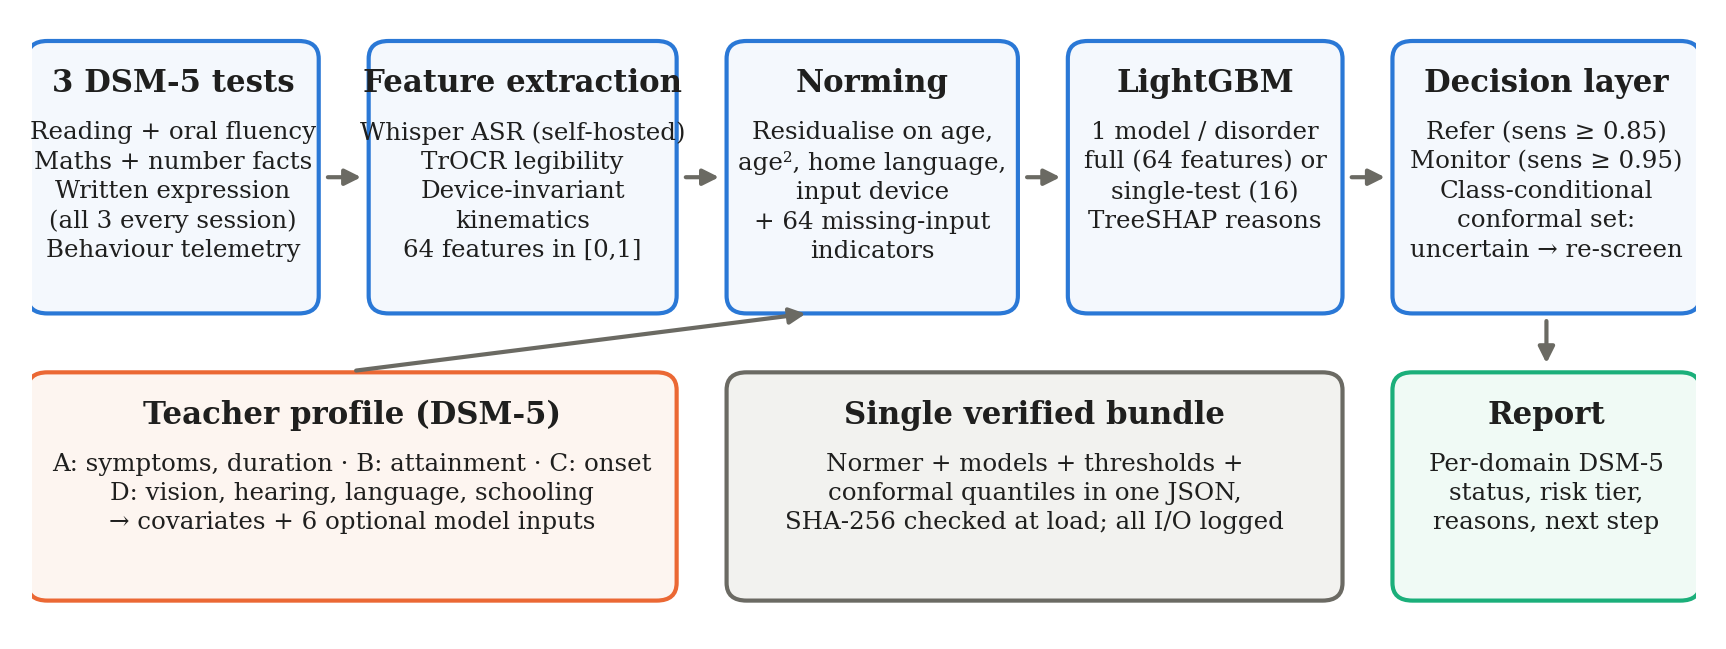
\includegraphics[width=0.92\textwidth]{fig1_system.png}
\caption{SwarSetu screening path. The three DSM-5 tests are converted into 64 features, normed for age, language and device, scored by one LightGBM model per disorder and mapped to referral tiers with conformal uncertainty. The teacher profile supplies covariates and DSM-5 Criteria A, C and D, which tests cannot observe.}
\label{fig:system}
\end{figure*}

\begin{table}[!t]
\centering
\caption{DSM-5 specifiers and the SwarSetu tasks that measure them. All three tests are given in every screening session; tasks added for DSM-5 alignment in bold.}
\label{tab:specifiers}
\footnotesize
\setlength{\tabcolsep}{3pt}
\begin{tabular}{@{}lp{2.5cm}p{4.1cm}@{}}
\toprule
Test & DSM-5 specifier & Task and measure \\
\midrule
\multirow{3}{*}{Reading} & Word reading accuracy & Phonological awareness, pseudowords; \textbf{passage word accuracy} \\
 & Reading rate/fluency & \textbf{Oral reading: words correct per minute} \\
 & Comprehension & Passage questions \\
\midrule
\multirow{4}{*}{Maths} & Number sense & Magnitude comparison, estimation, subitising \\
 & Arithmetic facts & \textbf{Number facts: correct/min, time per fact} \\
 & Fluent calculation & \textbf{Number facts: accuracy}; multi-step items \\
 & Math reasoning & Word problems, sequences \\
\midrule
\multirow{3}{*}{Writing} & Spelling accuracy & \textbf{Dictated words and sentence} \\
 & Grammar, punctuation & \textbf{Dictated sentence; composition} \\
 & Clarity/organisation & \textbf{Composition (teacher rating)} \\
\bottomrule
\end{tabular}
\end{table}

%=====================================================================
\section{Realistic Synthetic Cohorts}\label{sec:cohort}
%=====================================================================
\subsection{Why the original benchmark was too easy}
The original generator lowered all 16 features of a disorder's block by a constant and then min--max normalised the dataset. The stated effect size of 0.6 was applied in units whose noise SD was 0.3, so the median per-feature Cohen's $d$ was 1.50--1.63 and prevalence 16--21\% instead of 15\%. Logistic regression reached test AUROCs of 0.96--0.97, so the benchmark could not separate models.

\subsection{Generative model}
Each child has five correlated latent abilities: reading/phonology $R$, number sense $M$, graphomotor control $W$, executive attention $E$ and processing speed $S$ ($\rho_{RM}{=}0.55$, $\rho_{RW}{=}0.40$, others 0.25--0.40). Following the liability-threshold model, disorder $k$ is present when its liability falls below the prevalence quantile:
\begin{equation}
\ell_k = r\,\tilde z_k + \sqrt{1-r^2}\,\varepsilon_k,\qquad y_k=\mathbb{1}\!\left[\ell_k<\Phi^{-1}(\pi_k)\right],
\end{equation}
where $\tilde z_k$ is the standardised primary latent ($R$, $M$, or $0.85W{+}0.25R$), $r{=}0.9$ is diagnostic reliability and $\pi{=}(0.08,0.06,0.07)$. Every child therefore carries three labels, and comorbidity is not imposed but emerges from the latent correlations: $P(\text{DCL}\mid\text{DLX}){=}0.22$, $P(\text{DLX}\mid\text{DCL}){=}0.29$ and $P(\text{DLX}\mid\text{DGR}){=}0.30$, within published ranges~\cite{willcutt2013}.

The 64 features keep the semantics, polarity, defaults and formulas of the production extractors. Each is a noisy combination of one or more latents (loadings 0.15--0.75), with deliberate cross-domain loadings (word problems load on $M$ and $R$). Median per-feature effect sizes are $d{=}0.77$, 0.91 and 0.81 for the three disorders. The generator adds \emph{development} (skills rise 0.25\,SD per year, ages 7--13); \emph{home language} (60\% of children are Hindi-dominant and score 0.35\,SD lower on English phonological and comprehension items without a disorder); \emph{input device} (70\% use a finger, so pressure is unavailable and kinematics are noisier); \emph{measurement} effects (binomial item scores, a reading-speed ceiling, 8\% missing items, 10\% skipped modules filled with extractor defaults); and an imperfect \emph{reference standard} (10\% of cases labelled negative, 1\% of typical children positive). An external Site~B shifts every factor: younger children, 85\% Hindi-dominant, 95\% finger input, more noise and missing data, and 25\% higher prevalence. Because of label noise, an oracle that knows each child's latent abilities reaches only AUROC 0.89--0.91, the realistic ceiling for any model.

%=====================================================================
\section{Screening Pipeline}\label{sec:pipeline}
%=====================================================================
\textbf{Norming.} Psychometric tests are scored against age norms; we do the same statistically. On children with none of the three disorders, each feature $x_j$ is regressed on covariates $c=(a,a^2,h,f)$---age, age squared, Hindi-dominant and finger input---and the model receives the standardised residual
\begin{equation}
z_j = \bigl(x_j - \hat\beta_j^{\top} c\bigr)/\hat\sigma_j .
\end{equation}
A seven-year-old is thus compared with other seven-year-olds of the same language and device. Unknown covariates are imputed with training means, and 15\% of training covariates are masked so that the model learns that case.

\textbf{Model and training objective.} The 64 normed features plus 64 missing-input indicators feed one LightGBM classifier~\cite{ke2017} per disorder (300 trees, 7 leaves, learning rate 0.03, row/column subsampling 0.8/0.7). The three classifiers are trained on the same children, whose label vector $\mathbf y_i=(y_{i1},y_{i2},y_{i3})$ marks dyslexia, dyscalculia and dysgraphia, so a comorbid child is a positive example for several models. Booster $F_k$ minimises the regularised binary log-loss
\begin{equation}
\mathcal L_k=-\frac1n\sum_{i=1}^{n}\Bigl[y_{ik}\log p_{ik}+(1-y_{ik})\log(1-p_{ik})\Bigr]+\lambda\sum_{t}\lVert \mathbf w_t\rVert^2,
\end{equation}
with $p_{ik}=\sigma(F_k(\mathbf z_i))$, leaf weights $\mathbf w_t$ of tree $t$ and $\lambda{=}1$. All three models share the normer, features and stratified splits (stratified on the eight label combinations). The \emph{comprehensive} models use all 64 features and score every full three-test session; three \emph{single-test} models use only their 16-feature block for teacher-permitted single tests, replacing the original 0.5-fill strategy.

\textbf{Operating points and uncertainty.} On validation data we set, for each disorder, a \emph{refer} threshold at sensitivity $\geq$0.85 and a \emph{monitor} threshold at $\geq$0.95. For each class separately we compute split-conformal quantiles of the score $1-\hat p(\text{true class})$ ($\alpha{=}0.1$)~\cite{angelopoulos2021}; the prediction set $\{0\}$, $\{1\}$ or $\{0,1\}$ is reported as screen-negative, screen-positive or \emph{uncertain: re-screen}. TreeSHAP~\cite{lundberg2020} names the skills behind each result.

\textbf{Packaging.} Normer, models, thresholds and conformal quantiles are saved in one JSON bundle with a SHA-256 checksum verified against the extractors' feature names at load. Every input, feature vector, prediction and model version is stored with any later confirmed diagnosis, so real labelled data accumulate for re-training.

%=====================================================================
\section{DSM-5 Tests, Handwriting and Speech}\label{sec:dsm5}
%=====================================================================
DSM-5 requires (A) symptoms persisting for six months despite targeted help, (B) attainment well below age expectations, (C) onset in the school years, and (D) that difficulties are not better explained by intellectual disability, uncorrected vision or hearing, lack of proficiency in the language of instruction or inadequate instruction~\cite{dsm5}. The three tests address Criterion~B for their domain; a teacher profile records date of birth, home language, language of instruction, device and items for Criteria A, C and D. Age, language and device feed the model covariates, and six questionnaire items (symptom frequency and teacher-rated attainment for each of the three domains) enter as optional inputs.

\textbf{Reading.} The child reads a graded passage aloud for up to a minute; the transcript is aligned with the passage by a semi-global edit distance that lets the child stop anywhere and does not count repetitions, and words correct per minute (WCPM) are compared with published norms~\cite{hasbrouck2017}. \textbf{Mathematics.} One minute of grade-appropriate number facts gives facts per minute and retrieval time, alongside number-sense and reasoning items. \textbf{Written expression.} Copying (legibility) is separated from dictation (spelling), a dictated sentence (capitalisation, punctuation) and, from Grade~3, a short composition rated by the teacher. When handwriting is weak but spelling and composition are not, the report points to a motor-coordination check rather than an SLD.

\textbf{Device-invariant handwriting.} The original scorer computed tremor and precision on raw pointer samples; touch screens report 120--240 events per second, so pixel quantisation looked like tremor, and its chord/path ``precision'' penalised every curved letter. Each stroke is now resampled at 3\% of its own size; with $L_\sigma$ the path length after Gaussian smoothing of width $\sigma$, the jitter index $J=L_1/L_4-1$ measures high-frequency oscillation independently of sampling rate and letter size. Fluency (speed in letter-heights per second, halts, pauses) uses per-device expectations; layout uses the slope and scatter of letter baselines; legibility is $1-\text{CER}$ from a self-hosted TrOCR recogniser~\cite{li2023trocr}. Domains are weighted 0.40/0.25/0.20/0.15 (legibility, fluency, motor, layout).

\textbf{Speech} is transcribed by a self-hosted Whisper model~\cite{radford2023whisper}, so children's audio never leaves the school's server; silent clips return an empty transcript instead of a hallucinated one.

\textbf{Combining the criteria.} For each of the three domains the profile and the latest session give one of four statuses: \emph{consistent} with DSM-5 (refer), \emph{exclusion review} (a Criterion~D factor could explain the difficulty; address it and re-screen), \emph{partial} (missing criteria listed) or \emph{not indicated}. Criterion~D is applied per domain: limited proficiency in the language of instruction can explain reading and writing difficulties but not poor number sense.

%=====================================================================
\section{Evaluation Protocol}\label{sec:protocol}
%=====================================================================
For each of five seeds we generate a cohort ($n{=}6000$) with all three labels per child, split it 60/20/20 stratified on the eight label combinations, and generate a Site~B cohort ($n{=}3000$). We compare logistic regression (LR), LR with the three covariates, random forest, XGBoost, LightGBM on raw features, an MLP, the FT-Transformer retrained under a corrected protocol with ASL+Dice, with temperature scaling, and with binary cross-entropy (BCE), the production pipeline, and the originally deployed artefacts without retraining (D-rows). Every metric---AUROC, AUPRC, expected calibration error (ECE), and sensitivity, specificity and PPV at the validation-chosen refer threshold---is computed separately for dyslexia, dyscalculia and dysgraphia and then macro-averaged; means\,$\pm$\,SD are over seeds. Paired bootstrap intervals resample each seed's test set 1000 times. Learning curves train on 250--16{,}000 children; a sensitivity analysis varies one generator assumption at a time (22 settings, three seeds each). The deployed bundle is trained on 20{,}000 children and evaluated per disorder on a 4000-child held-out test set. For DSM-5, the generator is extended with Criterion~D factors (30\% still developing and 10\% with limited proficiency in the language of instruction; 5\% vision, 3\% hearing concerns) and simulated teacher ratings with halo and language bias. Reading fluency is tested with 2000 simulated readers per grade passed through a recogniser error model at word error rates (WER) of 0--20\%, and handwriting with synthetic writers at device-realistic sampling rates (neat on pen, touch and mouse; tremor, stop-start, size/drift and distorted profiles; three writers each).

%=====================================================================
\section{Results}\label{sec:results}
%=====================================================================
\begin{table*}[!t]
\centering
\caption{Test results macro-averaged over the three disorders and five seeds (mean\,$\pm$\,SD); operating point chosen on validation data for sensitivity\,$\geq$\,0.85. Ext.\ = distribution-shifted Site~B. D-rows: originally deployed artefacts, not retrained.}
\label{tab:main}
\footnotesize
\setlength{\tabcolsep}{3.6pt}
\begin{tabular}{lcccccccc}
\toprule
Model & AUROC & AUPRC & ECE & Sens. & Spec. & PPV & Ext.\ AUROC & Ext.\ Spec. \\
\midrule
\textbf{LightGBM, normed (ours)} & \textbf{\pmsd{0.858}{0.012}} & \textbf{\pmsd{0.429}{0.022}} & \textbf{\pmsd{0.017}{0.003}} & \pmsd{0.856}{0.021} & \textbf{\pmsd{0.685}{0.025}} & \textbf{\pmsd{0.178}{0.014}} & \textbf{\pmsd{0.846}{0.006}} & \textbf{\pmsd{0.654}{0.039}} \\
\quad same, covariates unknown & \pmsd{0.803}{0.006} & \pmsd{0.322}{0.014} & \pmsd{0.041}{0.006} & \pmsd{0.844}{0.020} & \pmsd{0.574}{0.026} & \pmsd{0.135}{0.008} & \pmsd{0.812}{0.003} & \pmsd{0.364}{0.032} \\
LR + covariates & \pmsd{0.851}{0.014} & \pmsd{0.397}{0.016} & \pmsd{0.226}{0.011} & \pmsd{0.867}{0.039} & \pmsd{0.658}{0.032} & \pmsd{0.166}{0.010} & \pmsd{0.839}{0.008} & \pmsd{0.638}{0.046} \\
Logistic regression & \pmsd{0.807}{0.013} & \pmsd{0.318}{0.025} & \pmsd{0.261}{0.009} & \pmsd{0.859}{0.030} & \pmsd{0.563}{0.032} & \pmsd{0.136}{0.007} & \pmsd{0.804}{0.007} & \pmsd{0.424}{0.042} \\
Random forest & \pmsd{0.810}{0.008} & \pmsd{0.310}{0.019} & \pmsd{0.035}{0.002} & \pmsd{0.833}{0.013} & \pmsd{0.603}{0.027} & \pmsd{0.143}{0.012} & \pmsd{0.817}{0.006} & \pmsd{0.416}{0.033} \\
XGBoost & \pmsd{0.796}{0.010} & \pmsd{0.302}{0.021} & \pmsd{0.096}{0.005} & \pmsd{0.849}{0.018} & \pmsd{0.542}{0.022} & \pmsd{0.128}{0.008} & \pmsd{0.793}{0.011} & \pmsd{0.398}{0.037} \\
LightGBM (raw features) & \pmsd{0.799}{0.012} & \pmsd{0.307}{0.026} & \pmsd{0.047}{0.002} & \pmsd{0.857}{0.028} & \pmsd{0.548}{0.022} & \pmsd{0.132}{0.007} & \pmsd{0.798}{0.009} & \pmsd{0.422}{0.035} \\
MLP & \pmsd{0.741}{0.007} & \pmsd{0.242}{0.018} & \pmsd{0.075}{0.004} & \pmsd{0.858}{0.021} & \pmsd{0.405}{0.029} & \pmsd{0.103}{0.005} & \pmsd{0.739}{0.007} & \pmsd{0.339}{0.033} \\
FT-Transformer (ASL+Dice) & \pmsd{0.804}{0.016} & \pmsd{0.317}{0.033} & \pmsd{0.275}{0.017} & \pmsd{0.837}{0.023} & \pmsd{0.586}{0.012} & \pmsd{0.138}{0.007} & \pmsd{0.810}{0.011} & \pmsd{0.424}{0.017} \\
\quad + temperature scaling & \pmsd{0.804}{0.016} & \pmsd{0.317}{0.033} & \pmsd{0.314}{0.014} & \pmsd{0.837}{0.023} & \pmsd{0.586}{0.012} & \pmsd{0.138}{0.007} & \pmsd{0.810}{0.011} & \pmsd{0.424}{0.017} \\
FT-Transformer (BCE) & \pmsd{0.810}{0.012} & \pmsd{0.333}{0.022} & \pmsd{0.021}{0.003} & \pmsd{0.846}{0.024} & \pmsd{0.587}{0.037} & \pmsd{0.141}{0.010} & \pmsd{0.819}{0.004} & \pmsd{0.420}{0.030} \\
\midrule
D1 Deployed FT, as served & \pmsd{0.691}{0.015} & \pmsd{0.189}{0.032} & \pmsd{0.195}{0.003} & \pmsd{0.852}{0.036} & \pmsd{0.327}{0.037} & \pmsd{0.090}{0.002} & \pmsd{0.674}{0.007} & \pmsd{0.261}{0.020} \\
D3 Deployed single test & \pmsd{0.764}{0.015} & \pmsd{0.274}{0.019} & \pmsd{0.192}{0.003} & \pmsd{0.847}{0.029} & \pmsd{0.475}{0.040} & \pmsd{0.114}{0.005} & \pmsd{0.764}{0.004} & \pmsd{0.303}{0.047} \\
D4 Random-weight NN & \pmsd{0.475}{0.013} & \pmsd{0.096}{0.008} & \pmsd{0.654}{0.002} & \pmsd{0.833}{0.035} & \pmsd{0.103}{0.024} & \pmsd{0.068}{0.001} & \pmsd{0.492}{0.011} & \pmsd{0.123}{0.027} \\
\bottomrule
\end{tabular}
\end{table*}

\subsection{Discrimination and significance}
Table~\ref{tab:main} gives the macro-averaged comparison. Once retrained correctly, the FT-Transformer is no better than simple baselines: 0.804 (ASL+Dice) and 0.810 (BCE) against 0.807 for LR; early stopping selected weights from about epoch~2 in every run, so the network overfits 3600 children almost immediately. The production pipeline reaches 0.858. Paired bootstrap differences against every model are positive: +0.051 [0.043, 0.059] over LR, +0.048 [0.040, 0.057] over random forest, +0.062 [0.053, 0.071] over XGBoost, +0.053 [0.045, 0.063] and +0.048 [0.040, 0.057] over the ASL and BCE FT-Transformers (all $P{<}0.001$), and a small but consistent +0.007 [0.002, 0.012] over LR with the same covariates ($P{=}0.001$). On Site~B its AUROC falls by only 0.012 and specificity at the transported threshold stays at 0.65, whereas unadjusted models fall to about 0.42. Without age and language information the pipeline drops to 0.803: the application must collect these covariates.

\subsection{Results for each disorder}
Table~\ref{tab:perdis} reports the deployed bundle for each disorder separately. The comprehensive model reaches AUROC 0.855, 0.853 and 0.859 for dyslexia, dyscalculia and dysgraphia, and exceeds the FT-Transformer for every disorder by 0.04--0.07. Each disorder model is calibrated (ECE $\leq$0.012), meets the sensitivity target except dysgraphia (0.825, set on validation data and transported to test), and has an NPV of 0.98--0.99. Conformal sets cover 0.94--0.95 of affected children for dyslexia and dyscalculia but 0.88 for dysgraphia, slightly below the 0.90 target, reflecting the finite positive calibration sample (about 290 children). Single-test models lose at most 0.004 AUROC against the comprehensive model, but only the full three-test session can reveal co-occurring difficulties in another domain.

Fig.~\ref{fig:train} (left, middle) shows the training dynamics of all three disorder models. Training log-loss keeps falling, while validation log-loss reaches its minimum after 129, 142 and 184 iterations for dyslexia, dyscalculia and dysgraphia (mean over five seeds) and then rises by only about 0.003 by iteration 300; validation AUROC plateaus for every disorder, so the small trees and low learning rate prevent harmful overfitting. LightGBM is also best at every training size (Fig.~\ref{fig:train}, right): with 250 children it reaches 0.811, against 0.760 for LR with covariates and 0.697 for the FT-Transformer, which still trails at 16{,}000 (0.828 vs.\ 0.868). Real learning-disability datasets are small, so this regime matters most.

\begin{table*}[!t]
\centering
\caption{Per-disorder results of the deployed bundle (trained on 20{,}000 children, 4000-child held-out test set). Comprehensive = three-test session; single = teacher-permitted single test. Coverage = class-conditional conformal coverage for affected/unaffected children. Best iteration = minimum of validation log-loss (mean over five seeds). Last two columns: AUROC of baselines on the five-seed benchmark.}
\label{tab:perdis}
\footnotesize
\setlength{\tabcolsep}{4pt}
\begin{tabular}{lcccccccccccc}
\toprule
 & \multicolumn{2}{c}{AUROC} & & & \multicolumn{4}{c}{At refer threshold} & & & \multicolumn{2}{c}{Baseline AUROC} \\
\cmidrule(lr){2-3}\cmidrule(lr){6-9}\cmidrule(lr){12-13}
Disorder & Compr. & Single & AUPRC & ECE & Sens. & Spec. & PPV & NPV & Coverage & Best iter. & LR + cov. & FT (ASL) \\
\midrule
Dyslexia & 0.855 & 0.855 & 0.421 & 0.012 & 0.878 & 0.639 & 0.178 & 0.983 & 0.95/0.90 & 129 & 0.857 & 0.808 \\
Dyscalculia & 0.853 & 0.851 & 0.403 & 0.009 & 0.858 & 0.675 & 0.151 & 0.986 & 0.94/0.91 & 142 & 0.850 & 0.817 \\
Dysgraphia & 0.859 & 0.855 & 0.426 & 0.008 & 0.825 & 0.736 & 0.197 & 0.982 & 0.88/0.91 & 184 & 0.845 & 0.789 \\
\bottomrule
\end{tabular}
\end{table*}

\begin{figure*}[!t]
\centering
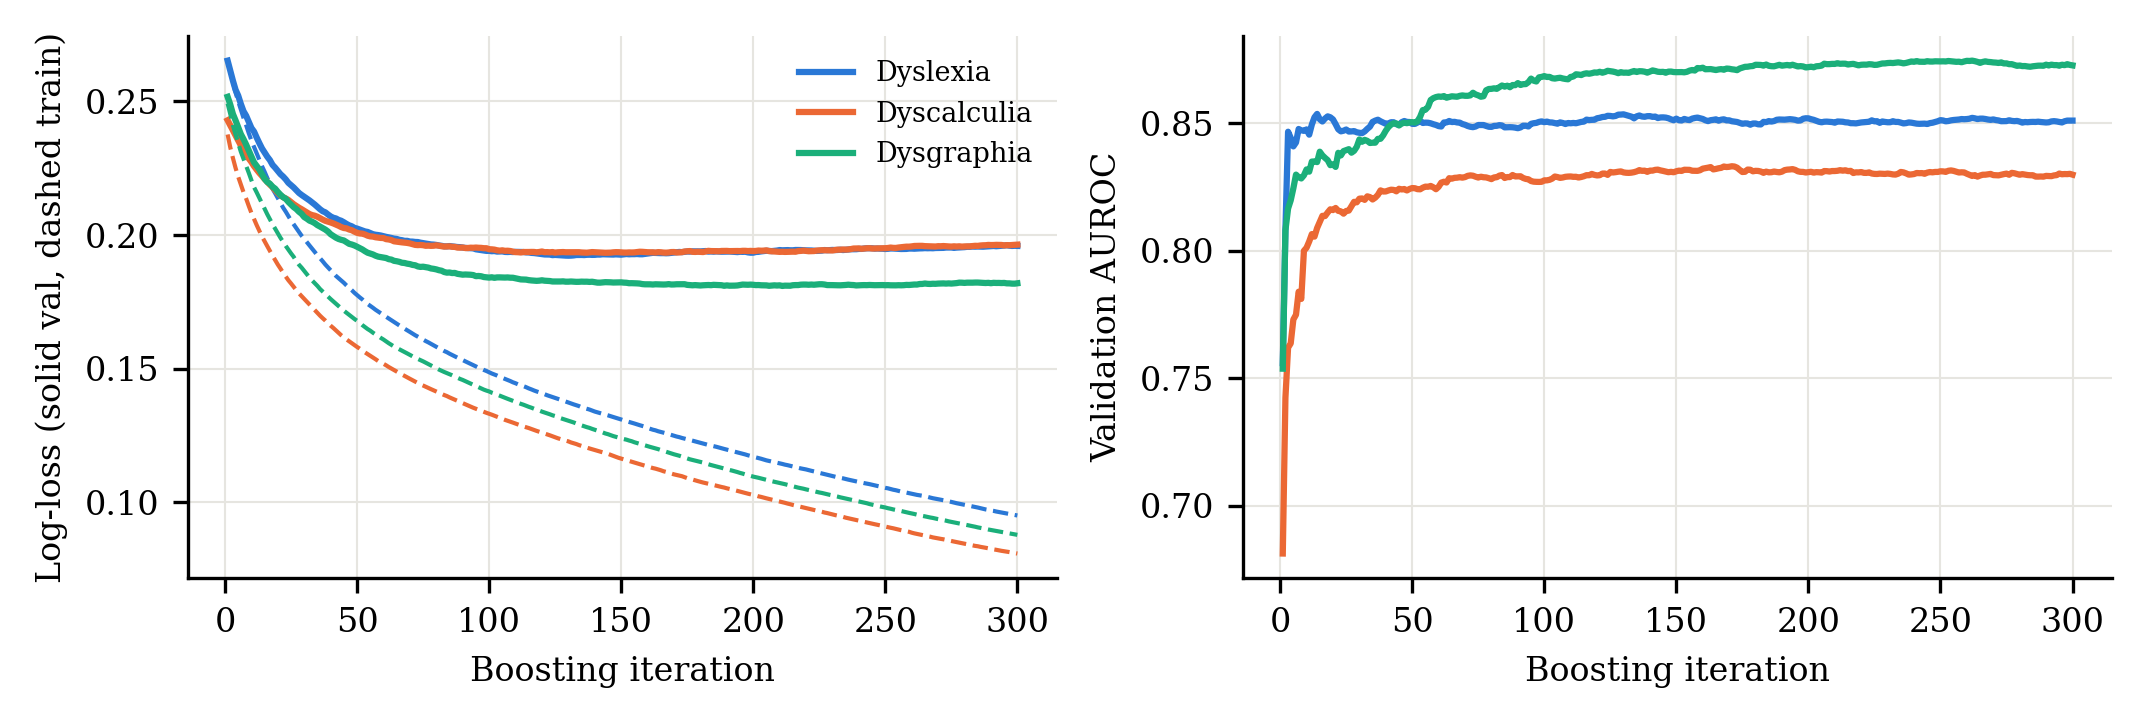
\includegraphics[width=0.64\textwidth]{fig2_boosting.png}\hfill
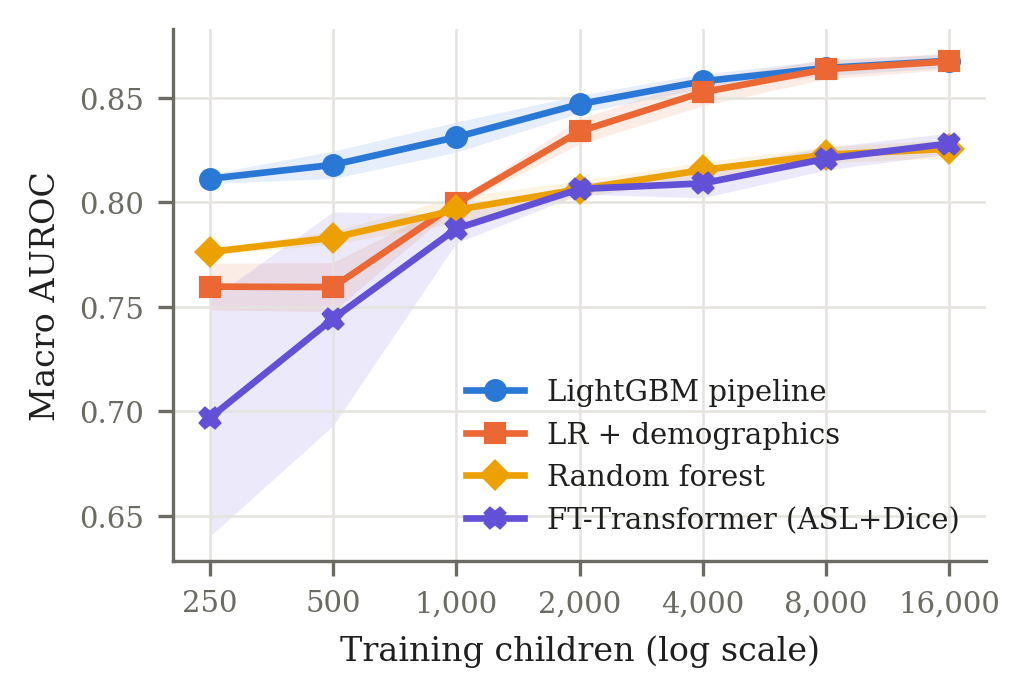
\includegraphics[width=0.33\textwidth]{fig2_learning_curves.png}
\caption{Training dynamics for all three disorders. Left: training (dashed) and validation (solid) log-loss; middle: validation AUROC per boosting iteration for the dyslexia, dyscalculia and dysgraphia models (seed~0). Right: macro AUROC versus training-set size (mean\,$\pm$\,SD, three seeds, fixed 6000-child test set).}
\label{fig:train}
\end{figure*}

\subsection{Sensitivity to the generator}
Because we designed the generator, Fig.~\ref{fig:sens} varies each assumption. The pipeline is best, or within 0.005 of the best model, in all 22 settings; it beats the ASL FT-Transformer in 22/22 and the BCE FT-Transformer in 21/22, and the ranking is stable (mean Kendall $\tau{=}0.89$). With no age effect, however, all models converge to 0.84--0.85: the advantage comes mainly from \emph{norming away the age and language confounds}, not from the learning algorithm.

\begin{figure*}[!t]
\centering
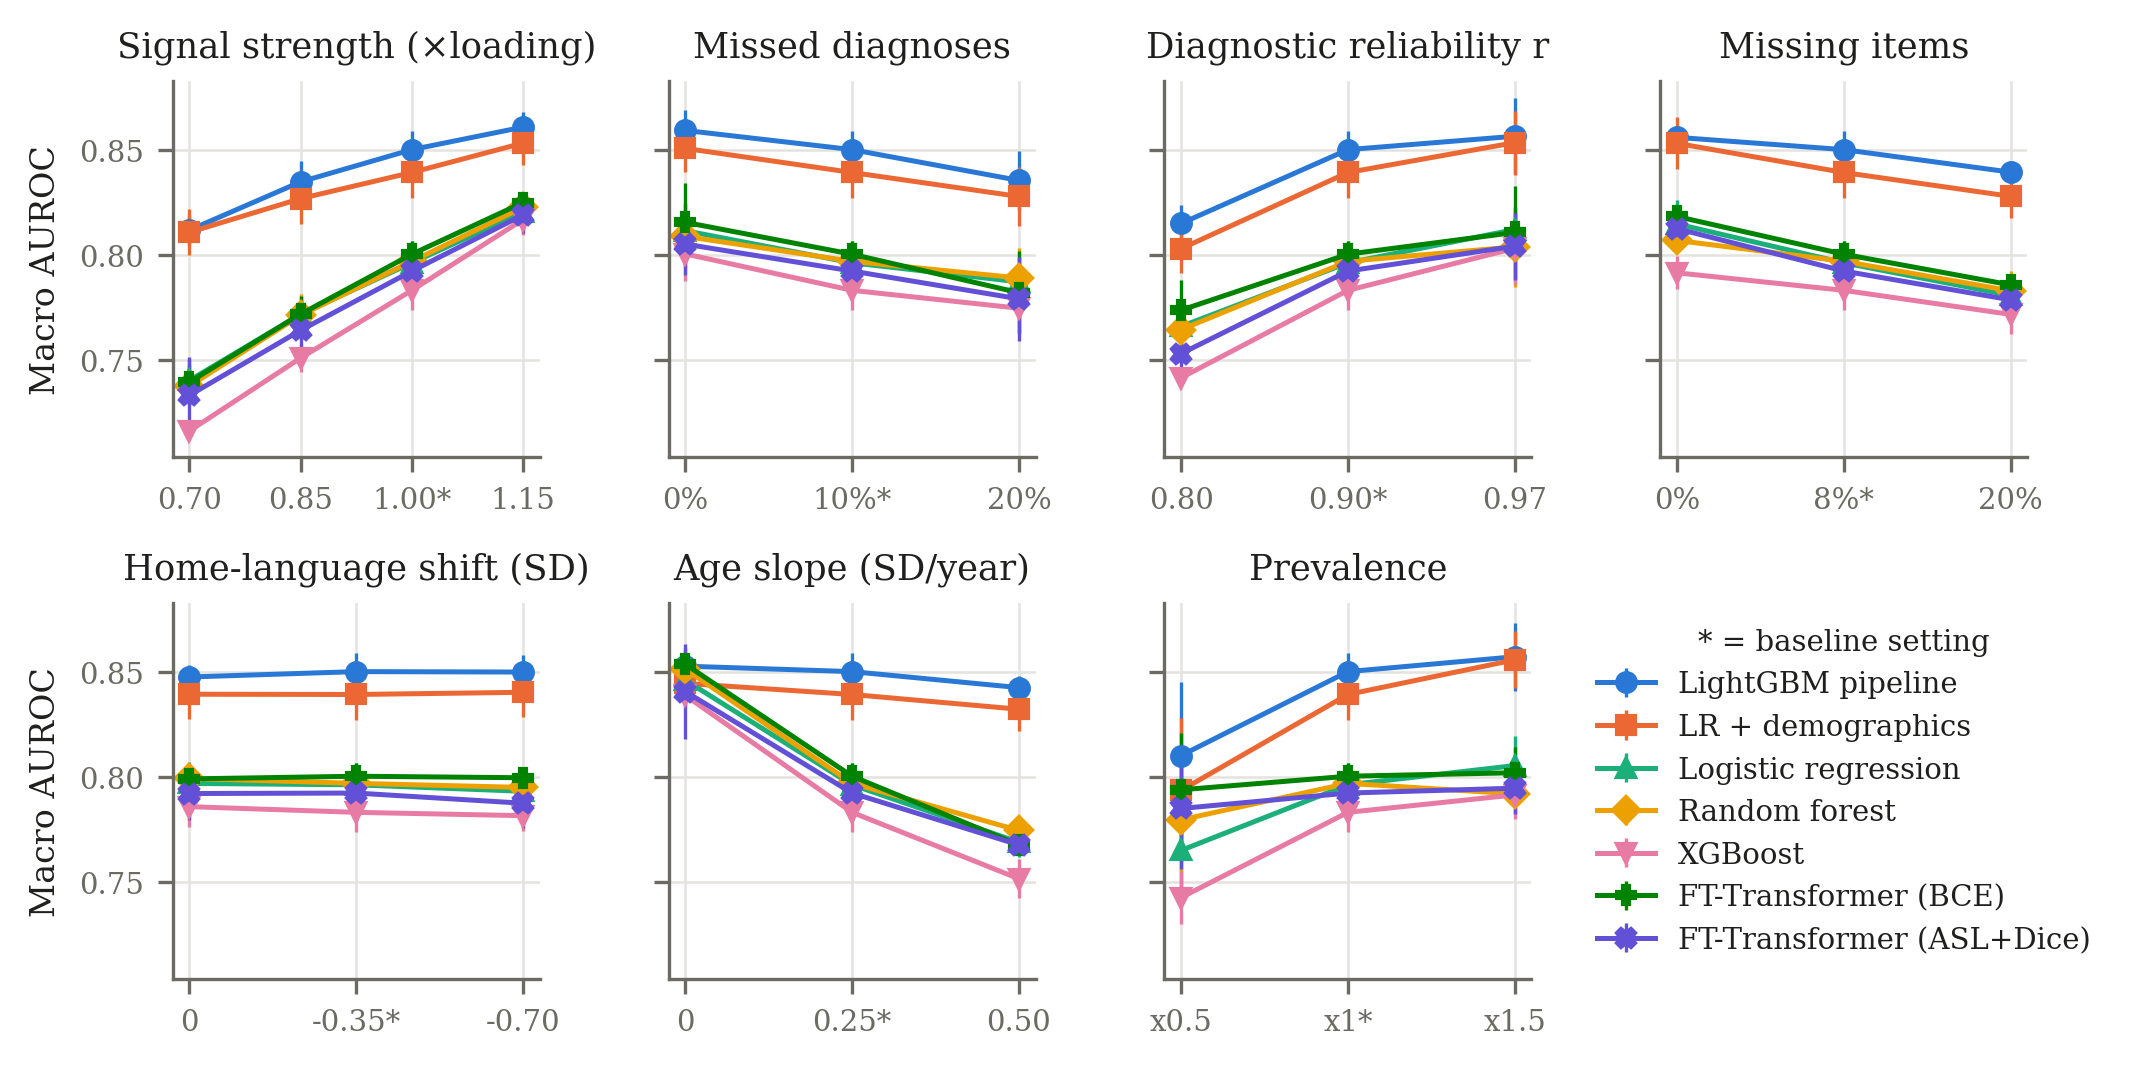
\includegraphics[width=0.9\textwidth]{fig3_sensitivity.png}
\caption{Generator sensitivity analysis: macro AUROC over the three disorders (mean\,$\pm$\,SD, three seeds) as one assumption is varied at a time; * marks the baseline setting.}
\label{fig:sens}
\end{figure*}

\subsection{Operating point, calibration and uncertainty}
At macro sensitivity 0.86 the pipeline has specificity 0.685, PPV 0.178 and NPV 0.984 at a prevalence of 6--8\%. In a school of 500 children this means about 180 referrals per disorder (34 true and 145 false positives) to find 34 of the 40 affected children; the tool is a first, high-sensitivity stage that rules children out, not a referral trigger on its own. Probabilities are calibrated without post-processing (ECE 0.017). ASL shifts probabilities upward (ECE 0.275) and temperature scaling makes this worse (0.314), because one temperature rescales logits but cannot remove a bias. The originally deployed ``90\% guaranteed'' intervals, with hard-coded widths, covered 0\% of test children; standard split-conformal sets covered 90\% overall but only 52--64\% of affected children, whereas class-conditional sets cover 0.94 of affected and 0.90 of unaffected children.

\subsection{Missing data and fairness}
With up to 40\% additional items removed at test time the pipeline falls from 0.858 to 0.813, degrading less than LR (to 0.757) and staying ahead of every model (Fig.~\ref{fig:missfair}a). Without covariates, Hindi-dominant children without dyslexia were flagged more often than English-dominant ones (false-positive rate 0.48 vs.\ 0.38 for the FT-Transformer) and 7--8-year-olds far more often than 11--12-year-olds (0.62 vs.\ 0.25; Fig.~\ref{fig:missfair}b). Adjustment narrows both gaps: for the deployed bundle, false-positive rates for English- vs.\ Hindi-dominant children are 0.32 vs.\ 0.39 (dyslexia), 0.32 vs.\ 0.33 (dyscalculia) and 0.25 vs.\ 0.27 (dysgraphia), and the age gap shrinks to 0.40 vs.\ 0.31 for dyslexia.

\begin{figure*}[!t]
\centering
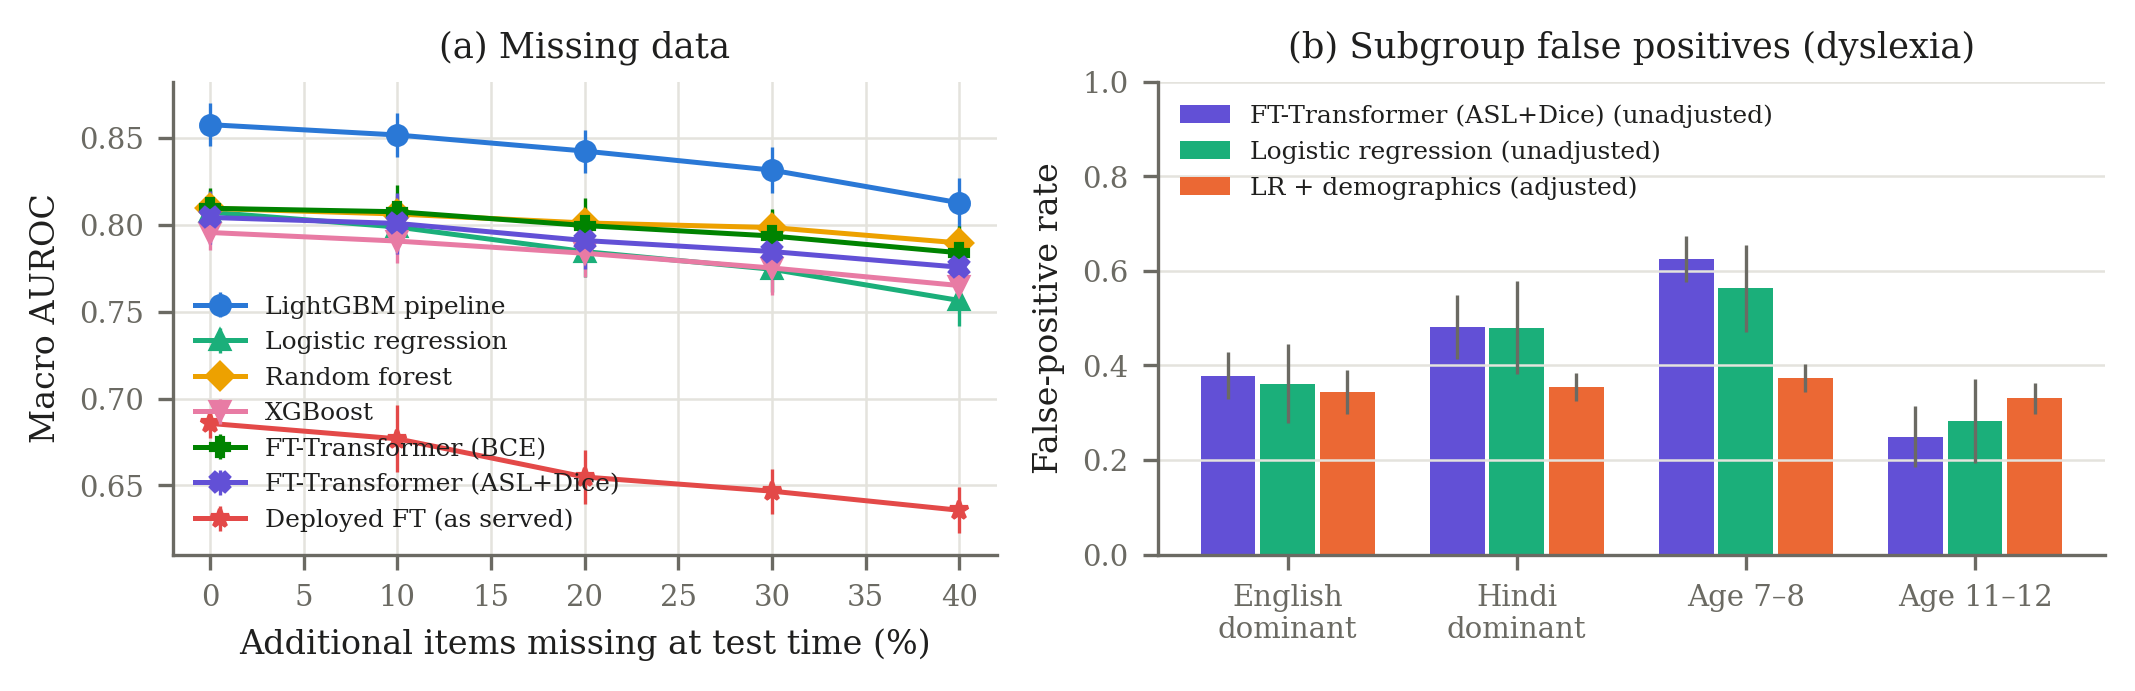
\includegraphics[width=0.85\textwidth]{fig4_missing_fairness.png}
\caption{(a) Macro AUROC as additional items are removed at test time (mean\,$\pm$\,SD, five seeds). (b) Dyslexia false-positive rate among children without dyslexia, by home language and age, for unadjusted and covariate-adjusted models.}
\label{fig:missfair}
\end{figure*}

\subsection{Handwriting}
The original scorer gave neat writing 85--86/100 on a 60\,Hz pen but only 60--62 on a touch screen and 54--56 with a mouse---below its scores for tremor (78--82): it was measuring the device (Table~\ref{tab:hw}). The new scorer gives all nine neat writers 99--100 and low risk on every device, flags all nine tremor, stop-start and layout writers and 2 of 3 distorted writers, and in each case its lowest domain matches the simulated deficit.

\begin{table}[!t]
\centering
\caption{Dysgraphia scores (0--100, three writers per profile), original vs.\ new analysis; risk L/M/H = low/moderate/high.}
\label{tab:hw}
\footnotesize
\setlength{\tabcolsep}{3pt}
\begin{tabular}{@{}lccc@{}}
\toprule
Profile & Original & New (risk) & Legibility \\
\midrule
Neat, pen (60\,Hz) & 85--86 & 100 (L,L,L) & 1.00 \\
Neat, touch (144\,Hz) & 60--62 & 100 (L,L,L) & 1.00 \\
Neat, mouse & 54--56 & 99--100 (L,L,L) & 1.00 \\
Tremor & 78--82 & 72--78 (M,H,H) & 0.70 \\
Stop-start & 56--58 & 86--90 (M,M,M) & 1.00 \\
Size / drift & 81--84 & 75--86 (H,H,M) & 0.88 \\
Distorted letters & 69--72 & 75--88 (H,M,L) & 0.79 \\
\bottomrule
\end{tabular}
\end{table}

\subsection{DSM-5 profile and Criterion D}
Adding the questionnaire to the three tests does not improve discrimination (Table~\ref{tab:dsm5}): macro AUROC 0.859 vs.\ 0.858, a paired bootstrap difference of +0.001 (95\% CI $-0.002$ to 0.004). The questionnaire alone reaches only 0.743, so ratings cannot replace testing. Language learners without a disorder are still flagged more often than fluent children (36\% vs.\ 30\%), which is what Criterion~D is for. Applying a Criterion~D rule (refer only children without a recorded D factor in the flagged domain) cuts the refer rate from 35.5\% to 27.1\% and raises specificity from 0.684 to 0.760, but sensitivity falls from 0.860 to 0.681 while PPV barely moves (0.178 to 0.187). D factors are common in children with and without a disorder, so the rule must \emph{defer, not exclude}: such children are re-screened after the factor is addressed.

\begin{table}[!t]
\centering
\caption{DSM-5 profile evaluation, macro over the three disorders and five seeds. FPR at the refer threshold among children without the disorder.}
\label{tab:dsm5}
\footnotesize
\setlength{\tabcolsep}{2.5pt}
\begin{tabular}{@{}lcccccc@{}}
\toprule
Model & AUROC & Ext. & Spec. & PPV & \multicolumn{2}{c}{FPR} \\
 & & & & & fluent & learner \\
\midrule
Tests + questionnaire & \pmsd{0.859}{.015} & 0.849 & 0.684 & 0.178 & 0.302 & 0.360 \\
Tests only & \pmsd{0.858}{.013} & 0.842 & 0.680 & 0.177 & 0.309 & 0.356 \\
\quad quest.\ withheld & \pmsd{0.853}{.012} & -- & 0.664 & 0.170 & 0.323 & 0.377 \\
Questionnaire only & \pmsd{0.743}{.030} & 0.738 & 0.395 & 0.102 & 0.593 & 0.644 \\
LR + cov.\ (tests) & \pmsd{0.849}{.014} & 0.835 & 0.647 & 0.164 & 0.341 & 0.392 \\
\bottomrule
\end{tabular}
\end{table}

\subsection{Speech and oral reading fluency}
On 20 synthetic spoken sentences the self-hosted Whisper model made no word errors (median 0.44\,s per clip on a laptop GPU); these are clean adult voices, so this shows that the service works, not its accuracy for children. With a clean transcript the reading alignment recovers WCPM within 0.3--2.5 words per minute (Table~\ref{tab:orf}). Recognition errors look like reading errors, so WCPM is biased downward roughly in proportion to WER, while the ranking of readers is preserved ($r\geq0.98$); the below-25th-percentile flag keeps its sensitivity but its specificity falls to 0.89--0.95 at 10\% WER and 0.77--0.90 at 20\%. The recogniser's error rate must therefore be measured locally, especially for Hindi, and flagged readings confirmed by the teacher.

\begin{table}[!t]
\centering
\caption{WCPM recovered from 2000 simulated readers per cell by recogniser WER; sensitivity/specificity of the below-25th-percentile flag.}
\label{tab:orf}
\footnotesize
\setlength{\tabcolsep}{3pt}
\begin{tabular}{@{}llrrccc@{}}
\toprule
Grade & WER & Bias & MAE & $r$ & Sens. & Spec. \\
\midrule
1 & 0\% & $+0.2$ & 0.3 & 0.999 & 0.99 & 1.00 \\
 & 10\% & $-4.6$ & 4.6 & 0.992 & 0.99 & 0.95 \\
 & 20\% & $-9.5$ & 9.5 & 0.982 & 0.99 & 0.90 \\
3 & 0\% & $+1.7$ & 1.8 & 0.999 & 0.96 & 1.00 \\
 & 10\% & $-6.2$ & 6.5 & 0.995 & 1.00 & 0.92 \\
 & 20\% & $-13.8$ & 13.9 & 0.990 & 1.00 & 0.79 \\
5 & 0\% & $+2.4$ & 2.5 & 0.999 & 0.96 & 1.00 \\
 & 10\% & $-7.6$ & 8.1 & 0.995 & 1.00 & 0.89 \\
 & 20\% & $-18.2$ & 18.3 & 0.992 & 1.00 & 0.77 \\
\bottomrule
\end{tabular}
\end{table}

%=====================================================================
\section{Lessons from the Deployment Audit}\label{sec:audit}
%=====================================================================
Executable checks confirmed 17 defects in the originally deployed system. Three combined to stop the screen working: (1)~\emph{train/serve skew}~\cite{sculley2015}---the network was trained on standardised features but served raw $[0,1]$ values; (2)~\emph{artefact mismatch}---the checkpoint stored no thresholds, so the engine loaded threshold and temperature files from an earlier run; (3)~\emph{regime mismatch}---thresholds fitted on deterministic probabilities were applied to Monte-Carlo-dropout averages of tempered probabilities. Served scores lay between 0.22 and 0.33 while thresholds were 0.91--0.93, so the screen flagged \emph{no child}: through the public API a severely impaired simulated reader scored 0.264 and a strong reader 0.247, both ``Low''. Other defects included early stopping that restored the last epoch (a live \texttt{state\_dict} reference), an unreachable ``High'' tier, hard-coded conformal widths and fairness status, legacy predictors with untrained random weights (AUROC 0.475), and the over-easy benchmark generator.

We draw five lessons. (i)~Ship model, preprocessing and thresholds as one verified artefact. (ii)~Test behaviour end to end---that risk rises with impairment through the API---not only status codes. (iii)~Compare models at the same pre-registered operating point; at a fixed 0.5 threshold ASL's upward shift masqueraded as extra sensitivity. (iv)~Compute uncertainty and fairness claims from model outputs; never hard-code them. (v)~Check that each measure tracks the child, not the device. All fixes are covered by regression tests, including tests that every risk tier is reachable and that a partial battery cannot be scored as a full screen.

%=====================================================================
\section{Alignment with Indian Standards}\label{sec:india}
%=====================================================================
A screen deployed in Indian schools is judged against Indian law, clinical practice, curriculum and research ethics, not only against DSM-5. Table~\ref{tab:india} maps each standard to SwarSetu's design.

\begin{table*}[!t]
\centering
\caption{Indian standards relevant to SLD screening and how SwarSetu addresses them.}
\label{tab:india}
\footnotesize
\setlength{\tabcolsep}{4pt}
\begin{tabular}{@{}p{3.6cm}p{6.3cm}p{6.8cm}@{}}
\toprule
Standard & Requirement (relevant part) & SwarSetu \\
\midrule
RPwD Act 2016~\cite{rpwd2016} & SLD (dyslexia, dysgraphia, dyscalculia, dyspraxia, developmental aphasia) is a specified disability & Screens the three academic forms; motor-only handwriting difficulty is routed to a coordination check \\
DEPwD guidelines 2018, amended 2020~\cite{depwd2018} & Certification by a medical authority (psychiatrist added in 2020) using the NIMHANS SLD battery after vision, hearing and IQ checks; from age 8, re-certified at 14 and 18 & Never certifies or labels; outputs referral tiers. Under-8s receive only \emph{monitor/at risk}. NIMHANS battery is the study reference standard \\
RCI Act 1992 & Assessment by RCI-registered professionals & Teachers administer the screen; reference assessment by an RCI-registered clinical psychologist \\
IPS 2019, IACP 2020 guidelines~\cite{shah2019ips,iacp2020} & Team assessment; exclusion of sensory, intellectual and instructional causes & Teacher questionnaire records Criterion~D factors; such children are deferred and re-screened, not referred \\
NEP 2020; NCERT Learning Outcomes~\cite{ncert2017lo} & Early identification; grade-wise competencies & Grades 1--12 item bank at ten NCERT-aligned levels \\
NIPUN Bharat; FLS 2022~\cite{fls2022} & Foundational reading targets (about 60 words/min by Class 3); Grade 3 benchmarks in 20 languages & Words correct per minute enter the model age- and language-normed; the advisory flag still uses US norms (limitation) \\
PRASHAST~\cite{prashast2022}; DALI~\cite{dali2021} & National precedents for teacher screening & Complementary: adds performance testing of maths and writing, Classes 1--12 \\
ICMR ethical guidelines 2017~\cite{icmr2017} & IEC approval, parental consent and child assent & Required before any real child is screened; forms in Hindi and English \\
DPDP Act 2023, Rules 2025~\cite{dpdp2023} & Verifiable parental consent; no behavioural monitoring of children except exempted educational purposes & Behavioural features are used only for the school's educational assessment; speech and handwriting recognition run on the school's machine; the explanation service receives no name or identifier \\
\bottomrule
\end{tabular}
\end{table*}

\textbf{Screening, not certification.} Indian certification of SLD is reserved for a medical authority using a specified battery~\cite{depwd2018}. SwarSetu therefore never reports that a child ``has'' a disorder: it returns screen-negative, \emph{monitor}, \emph{refer for assessment}, \emph{exclusion review} or \emph{uncertain: re-screen}, and no intelligence test is attempted, since excluding intellectual disability belongs to the diagnostic stage. This places it at the same tier as PRASHAST, with which it can be chained: a PRASHAST SLD flag can trigger a SwarSetu session, and a SwarSetu referral leads to the certifying assessment.

\textbf{Validation protocol.} The prospective study we specify uses the Indian reference standard: the NIMHANS SLD battery and an intelligence test administered by an RCI-registered clinical psychologist blinded to the screen result, in every screened child rather than only in screen-positives, so that sensitivity is estimable. Diagnostic accuracy is reported (STARD~2015~\cite{stard2015}) for children aged 8 and above, where certification applies; younger children are followed up. Thresholds are frozen on development data before the test set is scored, and the study is registered with the Clinical Trials Registry--India before enrolment. Estimating a sensitivity of 0.85 within $\pm0.10$ requires about 50 confirmed cases per disorder, i.e.\ 500--1000 school children at 5--10\% prevalence or fewer with clinic enrichment, whose spectrum bias is reported. The item bank is validated first: an expert panel rates content validity per grade, and a pilot estimates item difficulty (target 60--85\% correct for typical children) and discrimination. The research store and export tools already record each screen with model and item-bank version and import blinded clinician labels.

%=====================================================================
\section{Discussion and Limitations}\label{sec:discussion}
%=====================================================================
On data that reflects real measurement conditions, the transformer, asymmetric loss and label-correlation layer add complexity without improving accuracy. What helps is \emph{measuring the child correctly}: three DSM-5-based tests given together, norming for age and language, explicit handling of missing inputs, calibration before thresholding, uncertainty guarantees for the affected class, and handwriting measures that do not depend on the device. Three practical points follow. First, the application must collect age and home language; without them AUROC falls by 0.055 and external specificity halves. Second, at sensitivity 0.85 a single-stage screen refers many children (PPV 0.18), so it belongs at the first stage of a stepped pathway. Third, DSM-5 alignment changes \emph{what the screen says} more than how well it ranks children: the questionnaire records what tests cannot observe and stops the screen from treating a child who is still learning the language of instruction, or who needs glasses, as a likely case of dyslexia.

\textbf{Limitations.} All results are synthetic. The latent structure, loadings, confound sizes and noise levels are literature-informed choices, not estimates from SwarSetu data; the sensitivity analysis shows the ranking is robust within the ranges tested, but real data may contain effects we did not model. Handwriting thresholds need grade- and device-specific norms from real children, and the recogniser does not read Devanagari. The speech check used clean adult speech, and recogniser accuracy on Indian children's speech must be measured per language. The advisory reading-fluency flag uses US English norms~\cite{hasbrouck2017}; Indian benchmarks exist only for the foundational grades (NIPUN Bharat, FLS~2022~\cite{fls2022}), so local norms will come from the study. The NCERT-aligned item bank has content alignment but not yet content validity or item statistics. Only English and Hindi are supported, against 22 scheduled languages. The DSM-5 questionnaire has not been validated for reliability or agreement with specialists. Absolute numbers must not be quoted as clinical accuracy: a prospective study with blinded specialist assessment, ethics approval and parental consent is required before clinical use. The system already logs every assessment with its model version and accepts confirmed diagnoses for that purpose.

%=====================================================================
\section{Conclusion}
%=====================================================================
We replaced an over-easy benchmark with a realistic one and used it to build and stress-test a joint screen in which every session gives three DSM-5-based tests for reading, mathematics and written expression. A LightGBM pipeline on age- and language-normed features beat every alternative, including the originally proposed FT-Transformer, for each of the three disorders and on average, with statistically clear margins; it was calibrated, gave class-conditional coverage guarantees, narrowed subgroup gaps and held its advantage across 22 variations of the generator. The audit shows that for such systems, measurement validity and pipeline integrity matter more than model architecture.

\section*{Data and Code Availability}
Cohort generator and pipeline: \texttt{backend/screening/}; evaluations: \texttt{backend/reports/realistic\_eval/}; screening protocol: \texttt{frontend/src/lib/screeningBattery.ts}; handwriting analysis: \texttt{frontend/src/lib/dysgraphiaAnalysis.ts}; NCERT-aligned item bank: \texttt{frontend/src/lib/ncertItemBank.ts}; research export, labelling and evaluation: \texttt{backend/research\_cli.py}.

\section*{Acknowledgment}
[Funding and acknowledgements.] Following IEEE policy, we disclose that an AI assistant was used to help write code, run analyses and draft and edit the text; the authors reviewed all content and are responsible for it.

\begin{thebibliography}{99}
\bibitem{dsm5} American Psychiatric Association, \emph{Diagnostic and Statistical Manual of Mental Disorders}, 5th ed. Arlington, VA, USA: APA, 2013.
\bibitem{willcutt2013} E.~G. Willcutt \emph{et al.}, ``Comorbidity between reading disability and math disability: Concurrent psychopathology, functional impairment, and neuropsychological functioning,'' \emph{J. Learn. Disabil.}, vol.~46, no.~6, pp.~500--516, 2013.
\bibitem{rello2015} L.~Rello and M.~Ballesteros, ``Detecting readers with dyslexia using machine learning with eye tracking measures,'' in \emph{Proc. 12th Int. Web for All Conf. (W4A)}, 2015, pp.~1--8.
\bibitem{asselborn2018} T.~Asselborn \emph{et al.}, ``Automated human-level diagnosis of dysgraphia using a consumer tablet,'' \emph{npj Digit. Med.}, vol.~1, art.~42, 2018.
\bibitem{grinsztajn2022} L.~Grinsztajn, E.~Oyallon, and G.~Varoquaux, ``Why do tree-based models still outperform deep learning on typical tabular data?'' in \emph{Proc. NeurIPS Datasets and Benchmarks Track}, 2022.
\bibitem{gorishniy2021} Y.~Gorishniy, I.~Rubachev, V.~Khrulkov, and A.~Babenko, ``Revisiting deep learning models for tabular data,'' in \emph{Proc. NeurIPS}, 2021, pp.~18932--18943.
\bibitem{guo2017} C.~Guo, G.~Pleiss, Y.~Sun, and K.~Q. Weinberger, ``On calibration of modern neural networks,'' in \emph{Proc. ICML}, 2017, pp.~1321--1330.
\bibitem{angelopoulos2021} A.~N. Angelopoulos and S.~Bates, ``A gentle introduction to conformal prediction and distribution-free uncertainty quantification,'' arXiv:2107.07511, 2021.
\bibitem{sculley2015} D.~Sculley \emph{et al.}, ``Hidden technical debt in machine learning systems,'' in \emph{Proc. NeurIPS}, 2015, pp.~2503--2511.
\bibitem{benbaruch2021} E.~Ben-Baruch \emph{et al.}, ``Asymmetric loss for multi-label classification,'' in \emph{Proc. IEEE/CVF ICCV}, 2021, pp.~82--91.
\bibitem{ke2017} G.~Ke \emph{et al.}, ``LightGBM: A highly efficient gradient boosting decision tree,'' in \emph{Proc. NeurIPS}, 2017, pp.~3146--3154.
\bibitem{lundberg2020} S.~M. Lundberg \emph{et al.}, ``From local explanations to global understanding with explainable AI for trees,'' \emph{Nat. Mach. Intell.}, vol.~2, pp.~56--67, 2020.
\bibitem{hasbrouck2017} J.~Hasbrouck and G.~Tindal, ``An update to compiled ORF norms,'' Behavioral Research and Teaching, Univ. of Oregon, Eugene, OR, USA, Tech. Rep. 1702, 2017.
\bibitem{li2023trocr} M.~Li \emph{et al.}, ``TrOCR: Transformer-based optical character recognition with pre-trained models,'' in \emph{Proc. AAAI}, 2023, pp.~13094--13102.
\bibitem{radford2023whisper} A.~Radford \emph{et al.}, ``Robust speech recognition via large-scale weak supervision,'' in \emph{Proc. ICML}, 2023, pp.~28492--28518.
\bibitem{shah2019ips} H.~R. Shah \emph{et al.}, ``Clinical practice guidelines on assessment and management of specific learning disorders,'' \emph{Indian J. Psychiatry}, vol.~61, suppl.~2, pp.~211--225, 2019.
\bibitem{rpwd2016} Government of India, \emph{The Rights of Persons with Disabilities Act, 2016}, Act No.~49 of 2016.
\bibitem{depwd2018} Department of Empowerment of Persons with Disabilities, Ministry of Social Justice and Empowerment, ``Guidelines for the purpose of assessing the extent of specified disability in a person included under the RPwD Act, 2016,'' Gazette of India, 4 Jan.~2018; SLD provisions amended 9 Dec.~2020.
\bibitem{iacp2020} Indian Association of Clinical Psychologists, ``Practice guidelines for the assessment and intervention of specific learning disability,'' rev.~2020.
\bibitem{ncert2017lo} National Council of Educational Research and Training, \emph{Learning Outcomes at the Elementary Stage}. New Delhi, India: NCERT, 2017.
\bibitem{fls2022} Ministry of Education and NCERT, \emph{Foundational Learning Study 2022: Benchmarking Oral Reading Fluency and Numeracy in India}. New Delhi, India, 2022.
\bibitem{prashast2022} CIET--NCERT, ``PRASHAST: Pre assessment holistic screening tool---a disability screening checklist for schools,'' New Delhi, India, 2022.
\bibitem{dali2021} ``Development and standardization of the DALI-DAB dyslexia assessment battery for bilingual and biliterate children in India,'' \emph{Ann. Dyslexia}, 2021, doi:10.1007/s11881-021-00227-z.
\bibitem{icmr2017} Indian Council of Medical Research, \emph{National Ethical Guidelines for Biomedical and Health Research Involving Human Participants}. New Delhi, India: ICMR, 2017.
\bibitem{dpdp2023} Government of India, \emph{The Digital Personal Data Protection Act, 2023}, and \emph{Digital Personal Data Protection Rules, 2025}, G.S.R.~846(E).
\bibitem{stard2015} P.~M. Bossuyt \emph{et al.}, ``STARD 2015: An updated list of essential items for reporting diagnostic accuracy studies,'' \emph{BMJ}, vol.~351, art.~h5527, 2015.
\end{thebibliography}

\end{document}
